\documentclass[10pt,a4paper]{article}

% -----------------------------------------------------------------------------
% MATHS MANTHAN | Class 10 Arithmetic Progressions (AP) Handbook | 2026--27
% Self-contained publication-quality master formula & concept handbook.
% Strictly compliant with the rationalized CBSE Class 10 curriculum.
% Exactly 14 Pages with zero overfull boxes or unintended page overflow.
% -----------------------------------------------------------------------------

\usepackage[a4paper,top=12mm,bottom=15mm,left=15mm,right=15mm,footskip=8mm]{geometry}
\usepackage[T1]{fontenc}
\usepackage{lmodern}
\usepackage{microtype}
\usepackage{amsmath,amssymb}
\usepackage[table]{xcolor}
\usepackage{array,tabularx,booktabs}
\usepackage{graphicx}
\usepackage{eso-pic}
\usepackage{tikz}
\usetikzlibrary{calc,positioning,arrows.meta,shapes.geometric,patterns}
\usepackage[most]{tcolorbox}
\usepackage{enumitem}
\usepackage{fancyhdr}
\usepackage{lastpage}
\usepackage[hidelinks]{hyperref}
\usepackage{url}

% Compatibility fix for modern LaTeX/MiKTeX: colortbl + tabularx p-column alignment
\makeatletter
\let\insert@pcolumn\insert@column
\makeatother

% ============================================================================
% BRAND COLOR PALETTE — MATCHED TO THE MATHS MANTHAN STANDARD
% Primary navy: #001F49 | Brand gold: #D19029
% ============================================================================
\definecolor{primary}{RGB}{0,31,73}
\definecolor{brandnavy}{RGB}{0,31,73}
\definecolor{accent}{RGB}{209,144,41}
\definecolor{brandgold}{RGB}{209,144,41}
\definecolor{secondary}{RGB}{75,85,99}
\definecolor{lightgray}{RGB}{246,248,250}
\definecolor{accentlight}{RGB}{254,250,242}
\definecolor{primarylight}{RGB}{240,244,250}

\colorlet{navy}{primary}
\colorlet{blue}{primary!82!black}
\colorlet{gold}{accent}
\colorlet{goldpale}{accentlight}
\colorlet{bluepale}{primarylight}
\colorlet{ink}{secondary}
\colorlet{muted}{secondary}
\colorlet{linegray}{primary!25}
\colorlet{reddeep}{primary}
\colorlet{redpale}{lightgray}
\colorlet{green}{primary}
\colorlet{greenpale}{primarylight}

% Automatic low-opacity logo watermark on every page
\IfFileExists{mathsmanthan logo.png}{%
  \AddToShipoutPictureBG{%
    \begin{tikzpicture}[remember picture,overlay]
      \node[opacity=0.065] at (current page.center) {%
        \includegraphics[width=0.55\paperwidth,keepaspectratio]{mathsmanthan logo.png}%
      };
    \end{tikzpicture}%
  }%
}{}

\hypersetup{
  pdftitle={Class 10 Arithmetic Progressions | Maths Manthan Handbook},
  pdfauthor={Maths Manthan Tuition Classes},
  pdfsubject={CBSE Class 10 Mathematics, Academic Year 2026--27},
  pdfkeywords={Arithmetic Progressions, AP, nth term, Sum of AP, Common Difference, Arithmetic Mean, CBSE Class 10, Maths Manthan}
}

\setlength{\parindent}{0pt}
\setlength{\parskip}{1.8pt}
\renewcommand{\arraystretch}{1.12}
\setlist[itemize]{leftmargin=4.5mm,itemsep=0.8pt,topsep=0.8pt,parsep=0pt}
\setlist[enumerate]{leftmargin=5.2mm,itemsep=0.8pt,topsep=0.8pt,parsep=0pt}
\setlength{\tabcolsep}{4.5pt}
\emergencystretch=2em
\hfuzz=1pt

% ============================================================================
% HEADER / FOOTER
% ============================================================================
\newcommand{\TuitionName}{{\color{primary}MATHS} {\color{accent}MANTHAN}}
\newcommand{\TuitionSub}{{\color{primary}\textbullet\ \ \text{TUITION CLASSES}\ \ \textbullet}}
\newcommand{\ContactInfo}{e-mail: contact@mathsmanthan.co.in \quad$\vert$\quad Helpline: +91-8171546558}
\newcommand{\HandbookFooterTitle}{Class 10 Arithmetic Progressions Handbook}

\pagestyle{fancy}
\fancyhf{}
\renewcommand{\headrulewidth}{0pt}
\renewcommand{\footrulewidth}{0.6pt}
\renewcommand{\footrule}{\hbox to\headwidth{\color{primary!30}\leaders\hrule height 0.6pt\hfill}}
\fancyfoot[L]{\footnotesize\href{https://mathsmanthan.co.in}{\textcolor{secondary}{\TuitionName\ $\vert$\ \HandbookFooterTitle}}}
\fancyfoot[R]{\footnotesize\textbf{\color{primary}Page \thepage\ of \pageref{LastPage}}\quad\textcolor{accent}{\textbf{Academic Year 2026--27}}}

\fancypagestyle{plain}{%
  \fancyhf{}
  \fancyfoot[L]{\footnotesize\href{https://mathsmanthan.co.in}{\textcolor{secondary}{\TuitionName\ $\vert$\ \HandbookFooterTitle}}}
  \fancyfoot[R]{\footnotesize\textbf{\color{primary}Page \thepage\ of \pageref{LastPage}}\quad\textcolor{accent}{\textbf{Academic Year 2026--27}}}
  \renewcommand{\headrulewidth}{0pt}
  \renewcommand{\footrulewidth}{0.6pt}
  \renewcommand{\footrule}{\hbox to\headwidth{\color{primary!30}\leaders\hrule height 0.6pt\hfill}}
}

% Reusable design components
\newcommand{\BrandMark}{%
  \IfFileExists{mathsmanthan logo.png}{%
    \includegraphics[width=22mm,height=22mm,keepaspectratio]{mathsmanthan logo.png}%
  }{%
    
\begin{tikzpicture}[baseline=-0.6ex]
      \fill[navy,rounded corners=2.2pt] (0,0) rectangle (1.45,1.05);
      \draw[gold,line width=1.2pt] (0.15,0.15)--(1.30,0.15);
      \node[text=white,font=\sffamily\bfseries\Large] at (0.725,0.59) {MM};
    \end{tikzpicture}%
  }%
}

\newcommand{\chapterbanner}[4]{%
  \begin{tcolorbox}[enhanced,colback=bluepale,colframe=bluepale,boxrule=0pt,arc=2mm,
    left=3.5mm,right=3.5mm,top=1.6mm,bottom=1.6mm]
    {\footnotesize\bfseries\color{gold}CHAPTER #1\hfill\color{blue}#4}\par\vspace{0.3mm}
    {\Large\bfseries\color{navy}#2}\par
    {\small\color{muted}#3}
  \end{tcolorbox}\vspace{0.6mm}
}

\newcommand{\subhead}[1]{%
  \vspace{0.8mm}{\large\bfseries\color{navy}#1}\par\vspace{0.2mm}
  {\color{gold}\rule{14mm}{1.1pt}}\par\vspace{0.6mm}
}

\newtcolorbox{formulaBox}[1][]{enhanced,breakable,colback=goldpale,colframe=gold!65!black,
  boxrule=0.5pt,arc=1.5mm,left=2.5mm,right=2.5mm,top=1.5mm,bottom=1.5mm,
  before skip=1.8pt,after skip=2.2pt,#1}
\newtcolorbox{conceptBox}[1][]{enhanced,breakable,colback=bluepale,colframe=blue!25,
  boxrule=0.4pt,arc=1.5mm,left=2.5mm,right=2.5mm,top=1.5mm,bottom=1.5mm,
  before skip=1.8pt,after skip=2.2pt,#1}
\newtcolorbox{warningBox}[1][]{enhanced,breakable,colback=redpale,colframe=reddeep!45,
  boxrule=0.45pt,arc=1.5mm,left=2.5mm,right=2.5mm,top=1.5mm,bottom=1.5mm,
  before skip=1.8pt,after skip=2.2pt,#1}
\newtcolorbox{successBox}[1][]{enhanced,breakable,colback=greenpale,colframe=green!35,
  boxrule=0.45pt,arc=1.5mm,left=2.5mm,right=2.5mm,top=1.5mm,bottom=1.5mm,
  before skip=1.8pt,after skip=2.2pt,#1}

\newcommand{\CoreTag}{\tcbox[colback=greenpale,colframe=green!40,boxrule=.3pt,arc=1mm,left=1.5mm,right=1.5mm,top=.4mm,bottom=.4mm]{\scriptsize\bfseries\color{green}CORE SYLLABUS}}
\newcommand{\ExamTag}{\tcbox[colback=bluepale,colframe=blue!25,boxrule=.3pt,arc=1mm,left=1.5mm,right=1.5mm,top=.4mm,bottom=.4mm]{\scriptsize\bfseries\color{blue}EXAM STRATEGY}}
\newcommand{\TrapTag}{\tcbox[colback=redpale,colframe=reddeep!40,boxrule=.3pt,arc=1mm,left=1.5mm,right=1.5mm,top=.4mm,bottom=.4mm]{\scriptsize\bfseries\color{reddeep}TRAP ALERT}}
\newcommand{\ReferenceTag}{\tcbox[colback=bluepale,colframe=blue!25,boxrule=.3pt,arc=1mm,left=1.5mm,right=1.5mm,top=.4mm,bottom=.4mm]{\scriptsize\bfseries\color{blue}QUICK REFERENCE}}

\begin{document}

% =============================================================================
% PAGE 1: STANDALONE INSTITUTIONAL COVER PAGE
% =============================================================================
\thispagestyle{fancy}
\vspace*{0mm}
\noindent
\makebox[0pt][l]{%
  \raisebox{-0.80cm}[0pt][0pt]{%
    \href{https://mathsmanthan.co.in}{\BrandMark}%
  }%
}%
\parbox{\textwidth}{%
  \centering
  \href{https://mathsmanthan.co.in}{%
    {\fontsize{23pt}{23pt}\selectfont\bfseries \TuitionName}\\[3pt]
    {\footnotesize\bfseries \TuitionSub}%
  }\\[2pt]
  {\scriptsize\color{secondary} \ContactInfo}
}

\vspace{4pt}
\noindent{\color{primary}\rule{0.72\textwidth}{1.5pt}}\hfill{\color{accent}\rule{0.26\textwidth}{1.5pt}}

\vspace{2.5mm}
\begin{center}
  {\large\bfseries\color{muted}CBSE CLASS 10 \;$\vert$\; MATHEMATICS}\\[2.5mm]
  {\fontsize{26}{30}\selectfont\bfseries\color{navy}ARITHMETIC PROGRESSIONS}\\[1.8mm]
  {\Large\color{blue}Master Concept, Formula \& Visual Problem-Solving Handbook}\\[1.8mm]
  {\large\color{gold}\bfseries Academic Year 2026--27}
\end{center}

\vspace{2mm}

\begin{tikzpicture}
  \fill[navy,rounded corners=3mm] (0,0) rectangle (\textwidth,2.7);
  \draw[gold,line width=2pt] (0.35,0.35)--(0.35,2.35);
  \node[anchor=west,text=white,font=\bfseries\Large] at (0.7,2.15) {Every constant step builds infinity.};
  \node[anchor=west,text=white,font=\Large] at (0.7,1.65) {Master the discrete mathematics of linear patterns.};
  \node[anchor=west,text=white,font=\small] at (0.7,1.1) {General Term $a_n$ \;$\vert$\; Terminal Mechanics \;$\vert$\; Gauss's Sum $S_n$ \;$\vert$\; The Bridge $S_n \leftrightarrow a_n$ \;$\vert$\; Board Traps};
  \node[anchor=west,text=white!75,font=\footnotesize] at (0.7,0.55) {A student-first Maths Manthan conceptual and visual revision resource};
  
  \foreach \i/\h in {1/0.35, 2/0.65, 3/0.95, 4/1.25, 5/1.55, 6/1.85} {
    \fill[gold!85] (13.3 + \i*0.4, 0.4) rectangle (13.3 + \i*0.4 + 0.28, 0.4 + \h);
  }
  \draw[white, line width=1pt, -{Latex[scale=0.8]}] (13.5, 0.4) -- (16.0, 2.35);
\end{tikzpicture}

\vspace{2.5mm}
\begin{minipage}[t]{0.48\textwidth}
  \begin{conceptBox}[title=What This Handbook Includes,fonttitle=\bfseries\color{navy}]
    \begin{itemize}
      \item Sequence vs Series vs Arithmetic Progression
      \item General term derivation \& the fencepost principle
      \item Terminal mechanics: $n$-th term from end \& middle terms
      \item Arithmetic mean \& symmetric term selection techniques
      \item Gauss's forward-backward summation proof of $S_n$
      \item The telescoping bridge: $a_n = S_n - S_{n-1}$ \& degree hacks
      \item Double answer mechanics in decreasing series
      \item CBSE Section-E contextual case study archetypes
    \end{itemize}
  \end{conceptBox}
\end{minipage}\hfill
\begin{minipage}[t]{0.48\textwidth}
  \begin{formulaBox}[title=Pedagogical Strategy: Foundations First,fonttitle=\bfseries\color{navy}]
    \raggedright Arithmetic Progression is the discrete counterpart of the continuous linear function $y = mx + c$. The common difference $d$ represents constant slope, while $n$ is strictly quantized to positive integers:
    $$\mathbf{a_n = d \cdot n + (a - d) \;\longleftrightarrow\; y = m x + c}$$
    $$\mathbf{S_n = \left(\tfrac{d}{2}\right)n^2 + \left(a - \tfrac{d}{2}\right)n \;\longleftrightarrow\; \text{Linear Area}}$$
    Always state formulas with domain conditions: $\mathbf{n \in \{1, 2, 3, \dots\}}$.
  \end{formulaBox}
\end{minipage}

\vspace{1.5mm}
\begin{warningBox}[title=CBSE 2026--27 Curriculum Verification \& Rationalized Scope,fonttitle=\bfseries\color{navy}]
  \textbf{Official Scope (Prescribed \& Tested):} Motivation for studying AP, derivation of the $n$-th term ($a_n = a + (n-1)d$) and sum of first $n$ terms ($S_n = \frac{n}{2}[2a+(n-1)d] = \frac{n}{2}[a+l]$), their application in solving daily life contextual problems.\\
  \textbf{Excluded / Deleted Topics (Non-Examinable):}
  \begin{itemize}
    \item \textbf{Geometric Progressions (GP) \& Harmonic Progressions (HP):} Strictly outside Class 10 scope (covered in Class 11).
    \item \textbf{Sum of Squares ($\sum n^2$) and Sum of Cubes ($\sum n^3$):} Strictly non-examinable in Class 10.
    \item \textbf{Infinite Arithmetic Progressions Summation:} Only finite sums $S_n$ are evaluated.
    \item \textbf{Non-linear daily-life word problems:} Complex multi-equation systems not reducible to linear AP relations.
  \end{itemize}
\end{warningBox}

\vfill
\begin{center}
  {\small\bfseries\color{navy}Maths Manthan Tuition Classes}\\
  {\footnotesize\color{muted}contact@mathsmanthan.co.in \quad$\vert$\quad +91-8171546558}\\
  {\footnotesize\url{https://mathsmanthan.co.in}}\\[1.2mm]
  {\scriptsize\color{muted}Prepared for learning and conceptual mastery \;--\; Strictly aligned with CBSE Class 10 Syllabus 2026--27.}
\end{center}

\clearpage

% =============================================================================
% PAGE 2: MODULE 1 — FOUNDATIONAL ANATOMY: SEQUENCES, SERIES & COMMON DIFFERENCE
% =============================================================================
\thispagestyle{fancy}
\vspace*{0mm}

\chapterbanner{05}{ARITHMETIC PROGRESSIONS}{Module 1 $\vert$ Foundational Anatomy: Sequences, Series \& Common Difference}{\CoreTag}

\subhead{1.1 Hierarchy: Sequence, Series, and Progression}

\begin{itemize}
  \item \textbf{Sequence:} An ordered arrangement of numbers according to a definite rule: $a_1, a_2, a_3, \dots, a_n$. Each element is a \textbf{term}.
  \item \textbf{Series:} The indicated sum of the terms of a sequence: $a_1 + a_2 + a_3 + \dots + a_n$.
  \item \textbf{Arithmetic Progression (AP):} A sequence where each term after the first is obtained by adding a fixed constant $d$ to the preceding term.
\end{itemize}

\vspace{0.6mm}
\begin{minipage}[c]{0.52\textwidth}
\begin{formulaBox}
  \textbf{Formal Definition of an AP:}
  $$\mathbf{a_{k+1} - a_k = d \quad \text{for all } k \in \mathbb{N}}$$
  \textbf{The Three Regimes of Common Difference ($d \in \mathbb{R}$):}
  \begin{itemize}
    \item \textbf{$d > 0$ (Increasing AP):} $a_1 < a_2 < a_3 < \dots$ \par e.g., $3, 7, 11, 15, \dots$ ($d = +4$).
    \item \textbf{$d < 0$ (Decreasing AP):} $a_1 > a_2 > a_3 > \dots$ \par e.g., $20, 15, 10, 5, \dots$ ($d = -5$).
    \item \textbf{$d = 0$ (Stationary AP):} $a_1 = a_2 = a_3 = \dots$ \par e.g., $7, 7, 7, 7, \dots$ ($d = 0$).
  \end{itemize}
  \textit{Note: $d$ can be rational, irrational, positive, or negative.}
\end{formulaBox}
\end{minipage}\hfill
\begin{minipage}[c]{0.45\textwidth}
\centering
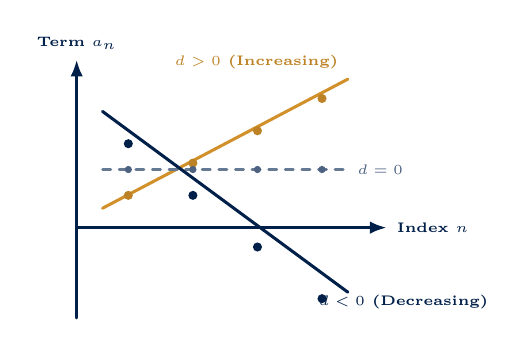
\begin{tikzpicture}[scale=0.82, line cap=round, line join=round]
  \draw[-{Latex[scale=0.8]}, primary, line width=1pt] (0,0) -- (4.8,0) node[right, font=\tiny\bfseries]{Index $n$};
  \draw[-{Latex[scale=0.8]}, primary, line width=1pt] (0,-1.4) -- (0,2.6) node[above, font=\tiny\bfseries]{Term $a_n$};

  % d > 0
  \draw[gold, line width=1.1pt] (0.4,0.3) -- (4.2,2.3);
  \foreach \x/\y in {0.8/0.5, 1.8/1.0, 2.8/1.5, 3.8/2.0} {
    \fill[gold!90!black] (\x,\y) circle (2pt);
  }
  \node[font=\tiny\bfseries\color{gold!90!black}, above left] at (4.2,2.3) {$d > 0$ (Increasing)};

  % d = 0
  \draw[primary!60, line width=0.9pt, dashed] (0.4,0.9) -- (4.2,0.9);
  \foreach \x in {0.8, 1.8, 2.8, 3.8} { \fill[primary!70] (\x,0.9) circle (1.6pt); }
  \node[font=\tiny\bfseries\color{primary!70}, right] at (4.2,0.9) {$d = 0$};

  % d < 0
  \draw[reddeep, line width=1.1pt] (0.4,1.8) -- (4.2,-1.0);
  \foreach \x/\y in {0.8/1.3, 1.8/0.5, 2.8/-0.3, 3.8/-1.1} {
    \fill[reddeep] (\x,\y) circle (2pt);
  }
  \node[font=\tiny\bfseries\color{reddeep}, below right] at (3.6,-0.9) {$d < 0$ (Decreasing)};
\end{tikzpicture}
\end{minipage}

\vspace{0.8mm}
\subhead{1.2 Deterministic Verification Protocol}

\begin{conceptBox}[title=Algorithmic AP Verification Protocol,fonttitle=\bfseries\color{navy}]
  \begin{itemize}
    \item \textbf{Explicit List of Terms ($a_1, a_2, a_3, \dots$):} Calculate consecutive differences $d_1 = a_2 - a_1, d_2 = a_3 - a_2, \dots$. The sequence is an AP if and only if $d_1 = d_2 = d_3 = \dots = d$ (constant).
    \item \textbf{Algebraic Formula ($a_n$):} Compute $a_{n+1}$ and evaluate $\Delta_n = a_{n+1} - a_n$. If $\Delta_n$ is a constant independent of $n$, it is an AP with common difference $d = \Delta_n$.
  \end{itemize}
\end{conceptBox}

\vspace{0.8mm}
\begin{conceptBox}[title={Worked Archetype 1 $\vert$ Algebraic and Radical AP Verification},fonttitle=\bfseries\color{navy}]
  \textbf{Problem:} (i) Is $a_n = 4n + 7$ an AP? (ii) Do $\sqrt{2}, \sqrt{8}, \sqrt{18}, \sqrt{32}, \dots$ form an AP?\\
  \textbf{Solution:}
  \begin{enumerate}
    \item $a_{n+1} = 4(n+1) + 7 = 4n + 11 \implies a_{n+1} - a_n = (4n+11) - (4n+7) = \mathbf{4}$ (Constant, independent of $n$).\\
      $\therefore$ The sequence is an AP with common difference $d = 4$ and first term $a_1 = 4(1)+7 = 11$.
    \item Simplify radicals: $a_1 = \sqrt{2}, a_2 = 2\sqrt{2}, a_3 = 3\sqrt{2}, a_4 = 4\sqrt{2}$.\\
      Consecutive differences: $a_2 - a_1 = \sqrt{2}, a_3 - a_2 = \sqrt{2}, a_4 - a_3 = \sqrt{2}$.\\
      $\because a_{k+1} - a_k = \sqrt{2} = \text{constant}$, the sequence \textbf{forms an AP with $a = \sqrt{2}$ and $d = \sqrt{2}$}.
  \end{enumerate}
\end{conceptBox}

\clearpage

% =============================================================================
% PAGE 3: MODULE 2 — THE GENERAL TERM (n-th TERM): a_n = a + (n-1)d
% =============================================================================
\thispagestyle{fancy}
\vspace*{0mm}

\chapterbanner{05}{ARITHMETIC PROGRESSIONS}{Module 2 $\vert$ The General Term: Inductive Derivation \& Fencepost Geometry}{\CoreTag}

\subhead{2.1 Inductive Derivation \& The Fencepost Principle}

Let an AP have first term $a$ and common difference $d$. Successive terms unfold inductively:
$$a_1 = a = a + (1-1)d, \quad a_2 = a + 1d = a + (2-1)d, \quad a_3 = a + 2d = a + (3-1)d$$
By mathematical induction, the coefficient of $d$ is always $1$ less than the position index:

\vspace{0.6mm}
\begin{minipage}[c]{0.45\textwidth}
\centering
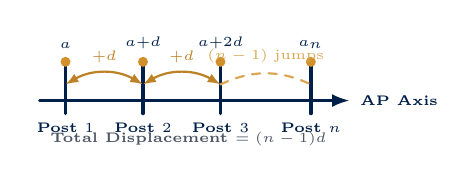
\begin{tikzpicture}[scale=0.82, line cap=round, line join=round]
  \draw[-{Latex[scale=0.8]}, primary, line width=1.1pt] (0,0) -- (4.8,0) node[right, font=\tiny\bfseries]{AP Axis};
  \foreach \x/\label/\term in {0.4/1/a, 1.6/2/a{+}d, 2.8/3/a{+}2d, 4.2/n/a_n} {
    \draw[primary, line width=1.3pt] (\x,-0.2) -- (\x,0.6);
    \fill[gold] (\x,0.6) circle (2.2pt);
    \node[below, font=\tiny\bfseries\color{primary}] at (\x,-0.2) {Post $\label$};
    \node[above, font=\tiny\bfseries\color{navy}] at (\x,0.65) {$\term$};
  }
  \draw[{Latex[scale=0.7]}-{Latex[scale=0.7]}, gold!90!black, line width=0.8pt] (0.4,0.25) to[bend left=30] node[midway, above, font=\tiny]{$+d$} (1.6,0.25);
  \draw[{Latex[scale=0.7]}-{Latex[scale=0.7]}, gold!90!black, line width=0.8pt] (1.6,0.25) to[bend left=30] node[midway, above, font=\tiny]{$+d$} (2.8,0.25);
  \draw[dashed, gold!80, line width=0.8pt] (2.8,0.25) to[bend left=25] node[midway, above, font=\tiny]{$(n-1)\text{ jumps}$} (4.2,0.25);
  \node[font=\tiny\bfseries\color{secondary}, align=center] at (2.3,-0.6) {Total Displacement $= (n-1)d$};
\end{tikzpicture}
\end{minipage}\hfill
\begin{minipage}[c]{0.52\textwidth}
\begin{formulaBox}
  \textbf{The General Term ($n$-th Term) Master Formula:}
  $$\mathbf{a_n = a + (n - 1)d}$$
  \begin{itemize}
    \item $\mathbf{a}$ = First term of the progression ($a = a_1$)
    \item $\mathbf{d}$ = Common difference ($d = a_{k+1} - a_k$)
    \item $\mathbf{n}$ = Term position ($\mathbf{n \in \mathbb{N} = \{1, 2, 3, \dots\}}$)
    \item $\mathbf{a_n}$ = Value of the $n$-th term (or last term $l$)
  \end{itemize}
  \textbf{The Fencepost Rule:} To build $n$ posts, exactly $(n-1)$ gaps are spanned. Hence $(n-1)$ additions of $d$ reach term $a_n$.
\end{formulaBox}
\end{minipage}

\vspace{0.8mm}
\subhead{2.2 The Linear Function Signature ($a_n = An + B$)}

Expanding the general term algebraically:
$$a_n = a + nd - d = \mathbf{d \cdot n + (a - d)}$$

\begin{formulaBox}
  \textbf{Linear Theorem of AP:}
  A sequence is an Arithmetic Progression if and only if its $n$-th term is a \textbf{linear polynomial in $n$}:
  $$\mathbf{a_n = An + B} \quad \implies \quad \mathbf{\text{Common Difference } d = A}, \quad \mathbf{\text{First Term } a = A + B}$$
  \textbf{MCQ Rule:} The coefficient of $n$ is \textbf{always} the common difference $d$!
\end{formulaBox}

\vspace{0.8mm}
\begin{conceptBox}[title={Worked Archetype 2 $\vert$ Position Membership and Domain Verification},fonttitle=\bfseries\color{navy}]
  \textbf{Problem:} (i) Which term of the AP: $3, 8, 13, 18, \dots$ is $78$? (ii) Is $301$ a term of $5, 11, 17, 23, \dots$?\\
  \textbf{Solution:}
  \begin{enumerate}
    \item Here, $a = 3$, $d = 8 - 3 = 5$. Set $a_n = 78$:
      $$3 + (n - 1)5 = 78 \implies 5(n - 1) = 75 \implies n - 1 = 15 \implies \mathbf{n = 16}$$
      $\therefore$ The \textbf{$16$-th term} of the AP is $78$.
    \item Here, $a = 5$, $d = 11 - 5 = 6$. Set $a_n = 301$:
      $$5 + (n - 1)6 = 301 \implies 6(n - 1) = 296 \implies n - 1 = \frac{148}{3} \implies n = \mathbf{\frac{151}{3} = 50\frac{1}{3}}$$
      \textbf{Conclusion:} Since position $n$ must be a natural number ($n \in \mathbb{N}$) and $\frac{151}{3} \notin \mathbb{N}$, \textbf{$301$ is NOT a term}.
  \end{enumerate}
\end{conceptBox}

\clearpage

% =============================================================================
% PAGE 4: MODULE 3 — TERMINAL MECHANICS: n-th TERM FROM END & MIDDLE TERMS
% =============================================================================
\thispagestyle{fancy}
\vspace*{0mm}

\chapterbanner{05}{ARITHMETIC PROGRESSIONS}{Module 3 $\vert$ Terminal Mechanics: $n$-th Term from the End \& Middle Term Protocols}{\CoreTag}

\subhead{3.1 The $n$-th Term from the End of a Finite AP}

Consider a finite AP with first term $a$, common difference $d$, and last term $l$:
$$a, \ a + d, \ a + 2d, \ \dots, \ l - 2d, \ l - d, \ l$$

\vspace{0.6mm}
\begin{minipage}[c]{0.45\textwidth}
\centering
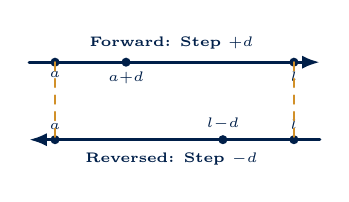
\begin{tikzpicture}[scale=0.82, line cap=round, line join=round]
  \draw[-{Latex[scale=0.8]}, primary, line width=1.1pt] (0,1.6) -- (4.5,1.6);
  \node[above, font=\tiny\bfseries\color{primary}] at (2.2,1.65) {Forward: Step $+d$};
  \fill[primary] (0.4,1.6) circle (2pt) node[below, font=\tiny\bfseries]{$a$};
  \fill[primary] (1.5,1.6) circle (2pt) node[below, font=\tiny\bfseries]{$a{+}d$};
  \fill[primary] (4.1,1.6) circle (2pt) node[below, font=\tiny\bfseries]{$l$};

  \draw[{Latex[scale=0.8]}-, reddeep, line width=1.1pt] (0,0.4) -- (4.5,0.4);
  \node[below, font=\tiny\bfseries\color{reddeep}] at (2.2,0.35) {Reversed: Step $-d$};
  \fill[reddeep] (0.4,0.4) circle (2pt) node[above, font=\tiny\bfseries]{$a$};
  \fill[reddeep] (3.0,0.4) circle (2pt) node[above, font=\tiny\bfseries]{$l{-}d$};
  \fill[reddeep] (4.1,0.4) circle (2pt) node[above, font=\tiny\bfseries]{$l$};

  \draw[dashed, gold, line width=0.8pt] (4.1,1.6) -- (4.1,0.4);
  \draw[dashed, gold, line width=0.8pt] (0.4,1.6) -- (0.4,0.4);
\end{tikzpicture}
\end{minipage}\hfill
\begin{minipage}[c]{0.52\textwidth}
\begin{formulaBox}
  \textbf{Master Formula: $n$-th Term from the End ($a'_n$):}
  $$\mathbf{a'_n = l - (n - 1)d}$$
  \textbf{Invariance Property:} The sum of the $n$-th term from the beginning and the $n$-th term from the end is \textbf{constant}:
  $$\mathbf{a_n + a'_n = a + l}$$
  \textbf{Position Equivalence:} In an AP of $m$ total terms, the $n$-th term from the end is the \textbf{$(m - n + 1)$-th term from the start}.
\end{formulaBox}
\end{minipage}

\vspace{0.8mm}
\subhead{3.2 Middle Term(s) Protocol for Finite APs}

To determine the middle term of an AP $a, a+d, \dots, l$, first calculate total terms: $\mathbf{m = \frac{l - a}{d} + 1}$.

\begin{tabularx}{\textwidth}{m{0.24\textwidth} | m{0.32\textwidth} | X}
\toprule
\rowcolor{bluepale}
\textbf{Total Terms ($m$)} & \textbf{Number of Middle Terms} & \textbf{Exact Position \& Formula} \\
\midrule
\textbf{Case 1: $m$ is ODD} & Exactly \textbf{ONE} middle term & Position: $\mathbf{k = \frac{m + 1}{2}}$ \par Value: $\mathbf{a_k = a + \left(\frac{m-1}{2}\right)d}$ \\
\midrule
\textbf{Case 2: $m$ is EVEN} & Exactly \textbf{TWO} middle terms & Positions: $\mathbf{k_1 = \frac{m}{2}}$ and $\mathbf{k_2 = \frac{m}{2} + 1}$ \\
\bottomrule
\end{tabularx}

\vspace{0.8mm}
\begin{conceptBox}[title={Worked Archetype 3 $\vert$ End-Term and Middle-Term Identification},fonttitle=\bfseries\color{navy}]
  \textbf{Problem:} Given the AP: $10, 7, 4, \dots, -62$. (i) Find the $11$-th term from the end. (ii) Find the middle term of the AP.\\
  \textbf{Solution:}
  \begin{enumerate}
    \item Here, $a = 10$, $d = 7 - 10 = -3$, and last term $l = -62$.
      Using the end-term formula for $n = 11$:
      $$a'_{11} = l - (11 - 1)d = -62 - (10)(-3) = -62 + 30 = \mathbf{-32}$$
    \item First find total terms $m$: $-62 = 10 + (m - 1)(-3) \implies -72 = -3(m - 1) \implies m - 1 = 24 \implies m = 25$.
      Since $m = 25$ is \textbf{ODD}, there is exactly one middle term at position:
      $$k = \frac{m + 1}{2} = \frac{25 + 1}{2} = \mathbf{13}$$
      Value of middle term $a_{13} = a + 12d = 10 + 12(-3) = 10 - 36 = \mathbf{-26}$.
  \end{enumerate}
\end{conceptBox}

\clearpage

% =============================================================================
% PAGE 5: MODULE 4 — ARITHMETIC MEAN & SYMMETRICAL SELECTION OF TERMS
% =============================================================================
\thispagestyle{fancy}
\vspace*{0mm}

\chapterbanner{05}{ARITHMETIC PROGRESSIONS}{Module 4 $\vert$ Arithmetic Mean \& Symmetrical Selection of Terms}{\CoreTag}

\subhead{4.1 The Three-Term Equilibrium Condition \& Arithmetic Mean}

If three quantities $a, b, c$ are in AP, the common difference is identical:
$$b - a = c - b \implies \mathbf{2b = a + c} \implies \mathbf{b = \frac{a + c}{2}}$$

\vspace{0.6mm}
\begin{minipage}[c]{0.45\textwidth}
\centering
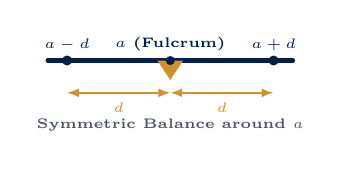
\begin{tikzpicture}[scale=0.82, line cap=round, line join=round]
  \draw[primary, line width=1.5pt] (0.4,1.3) -- (4.2,1.3);
  \fill[gold] (2.3,1.0) -- (2.1,1.3) -- (2.5,1.3) -- cycle;
  \fill[primary] (2.3,1.3) circle (2pt) node[above, font=\tiny\bfseries\color{navy}]{$a$ (Fulcrum)};
  \fill[reddeep] (0.7,1.3) circle (2.2pt) node[above, font=\tiny\bfseries\color{reddeep}]{$a-d$};
  \fill[reddeep] (3.9,1.3) circle (2.2pt) node[above, font=\tiny\bfseries\color{reddeep}]{$a+d$};
  \draw[{Latex[scale=0.7]}-{Latex[scale=0.7]}, accent, line width=0.7pt] (0.7,0.8) -- (2.3,0.8) node[midway, below, font=\tiny]{$d$};
  \draw[{Latex[scale=0.7]}-{Latex[scale=0.7]}, accent, line width=0.7pt] (2.3,0.8) -- (3.9,0.8) node[midway, below, font=\tiny]{$d$};
  \node[font=\tiny\bfseries\color{secondary}] at (2.3,0.3) {Symmetric Balance around $a$};
\end{tikzpicture}
\end{minipage}\hfill
\begin{minipage}[c]{0.52\textwidth}
\begin{formulaBox}
  \textbf{Symmetrical Variable Selection Protocol:}
  \begin{itemize}
    \item \textbf{3 Terms:} $\mathbf{a - d, \ a, \ a + d}$ \par (Common Diff $= \mathbf{d}$, Sum $= \mathbf{3a}$)
    \item \textbf{4 Terms:} $\mathbf{a - 3d, \ a - d, \ a + d, \ a + 3d}$ \par (Common Diff $= \mathbf{2d}$ \TrapTag, Sum $= \mathbf{4a}$)
    \item \textbf{5 Terms:} $\mathbf{a - 2d, \ a - d, \ a, \ a + d, \ a + 2d}$ \par (Common Diff $= \mathbf{d}$, Sum $= \mathbf{5a}$)
  \end{itemize}
  \textbf{Equilibrium:} Symmetrical terms cause $d$ to cancel completely upon summing!
\end{formulaBox}
\end{minipage}

\vspace{0.8mm}
\subhead{4.2 The 4-Term Common Difference Trap}

\begin{warningBox}
  \textbf{\TrapTag\ The 4-Term Common Difference Trap!}
  In the 4-term selection $(a - 3d, a - d, a + d, a + 3d)$, the difference between consecutive terms is $(a - d) - (a - 3d) = \mathbf{2d \ (\text{NOT } d!)}$. If you solve and get $d = 2$, the actual step of the AP is $\mathbf{2d = 4}$.
\end{warningBox}

\vspace{0.8mm}
\begin{conceptBox}[title={Worked Archetype 4 $\vert$ 3 Symmetrical Numbers in AP},fonttitle=\bfseries\color{navy}]
  \textbf{Problem:} The sum of three numbers in an AP is $27$ and their product is $648$. Find the numbers.\\
  \textbf{Solution:}
  \begin{enumerate}
    \item Let the three numbers in AP be $\mathbf{a - d, \ a, \ a + d}$.
    \item Sum condition: $(a - d) + a + (a + d) = 27 \implies 3a = 27 \implies \mathbf{a = 9}$.
    \item Product condition: $(a - d) \cdot a \cdot (a + d) = 648 \implies 9(81 - d^2) = 648 \implies 81 - d^2 = 72 \implies d^2 = 9 \implies \mathbf{d = \pm 3}$.
    \item For $d = 3$, numbers are $9 - 3, 9, 9 + 3 \implies \mathbf{6, 9, 12}$. For $d = -3$, numbers are $\mathbf{12, 9, 6}$.\\
      $\therefore$ The required numbers are \textbf{$6, 9, 12$}.
  \end{enumerate}
\end{conceptBox}

\clearpage

% =============================================================================
% PAGE 6: MODULE 5 — THE SUM OF FIRST n TERMS (S_n): GAUSS'S PROOF
% =============================================================================
\thispagestyle{fancy}
\vspace*{0mm}

\chapterbanner{05}{ARITHMETIC PROGRESSIONS}{Module 5 $\vert$ The Sum of First $n$ Terms: Gauss's Proof \& Dual Formulas}{\CoreTag}

\subhead{5.1 Gauss's Discovery \& The Forward-Backward Columnar Proof}

Writing the series forwards and backwards and adding column-wise:
\begin{align*}
  S_n &= a + (a + d) + (a + 2d) + \dots + l\\
  S_n &= l + (l - d) + (l - 2d) + \dots + a\\
  2S_n &= \underbrace{(a + l) + (a + l) + \dots + (a + l)}_{n \text{ identical pairs}} = n(a + l) \implies \mathbf{S_n = \frac{n}{2}(a + l)}
\end{align*}
Substituting $l = a + (n - 1)d$ yields: $\mathbf{S_n = \frac{n}{2}[2a + (n - 1)d]}$.

\vspace{0.6mm}
\begin{minipage}[c]{0.45\textwidth}
\centering
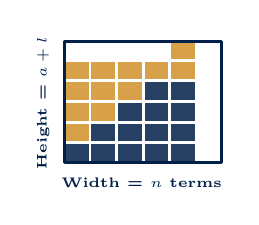
\begin{tikzpicture}[scale=0.75, line cap=round, line join=round]
  \foreach \i in {1,2,3,4,5} {
    \foreach \j in {1,...,\i} {
      \fill[primary!85] (\i*0.45, \j*0.35) rectangle (\i*0.45+0.4, \j*0.35+0.3);
    }
  }
  \foreach \i in {1,2,3,4,5} {
    \foreach \j in {\i,...,4} {
      \fill[gold!85] (\i*0.45, \j*0.35+0.35) rectangle (\i*0.45+0.4, \j*0.35+0.65);
    }
  }
  \draw[line width=1.1pt, primary] (0.45,0.35) rectangle (3.1,2.4);
  \node[font=\tiny\bfseries\color{primary}, below] at (1.75,0.25) {Width = $n$ terms};
  \node[font=\tiny\bfseries\color{primary}, rotate=90, above] at (0.35,1.35) {Height = $a+l$};
\end{tikzpicture}
\end{minipage}\hfill
\begin{minipage}[c]{0.52\textwidth}
\begin{formulaBox}
  \textbf{The Dual Master Sum Formulas:}
  $$\mathbf{S_n = \frac{n}{2}[2a + (n - 1)d]} \quad \longleftrightarrow \quad \mathbf{S_n = \frac{n}{2}[a + l]}$$
  \textbf{Standard Natural Number Summations:}
  \begin{itemize}
    \item First $n$ natural numbers: $\mathbf{\sum_{k=1}^n k = \frac{n(n + 1)}{2}}$
    \item First $n$ odd naturals: $\mathbf{1 + 3 + \dots + (2n-1) = n^2}$
    \item First $n$ even naturals: $\mathbf{2 + 4 + \dots + 2n = n(n + 1)}$
  \end{itemize}
\end{formulaBox}
\end{minipage}

\vspace{0.8mm}
\subhead{5.2 Direct Sum Applications}

\begin{conceptBox}[title={Worked Archetype 5 $\vert$ Direct Application of Sum Formulas},fonttitle=\bfseries\color{navy}]
  \textbf{Problem:} Find the sum of: (i) first $22$ terms of $8, 3, -2, \dots$ (ii) the series $34 + 32 + 30 + \dots + 10$.\\
  \textbf{Solution:}
  \begin{enumerate}
    \item Here, $a = 8$, $d = 3 - 8 = -5$, and $n = 22$.
      $$S_{22} = \frac{22}{2}[2(8) + (22 - 1)(-5)] = 11[16 + 21(-5)] = 11[16 - 105] = 11(-89) = \mathbf{-979}$$
    \item Here, $a = 34$, $d = 32 - 34 = -2$, and last term $l = 10$. First find $n$:
      $$10 = 34 + (n - 1)(-2) \implies -24 = -2(n - 1) \implies n - 1 = 12 \implies \mathbf{n = 13}$$
      Using the last-term formula: $S_{13} = \frac{13}{2}[a + l] = \frac{13}{2}[34 + 10] = \frac{13}{2}[44] = 13 \times 22 = \mathbf{286}$.
  \end{enumerate}
\end{conceptBox}

\clearpage

% =============================================================================
% PAGE 7: MODULE 6 — THE BRIDGE PRINCIPLE: CONNECTING S_n AND a_n
% =============================================================================
\thispagestyle{fancy}
\vspace*{0mm}

\chapterbanner{05}{ARITHMETIC PROGRESSIONS}{Module 6 $\vert$ The Bridge Principle: Connecting $S_n$ and $a_n$ \& Polynomial Degrees}{\CoreTag}

\subhead{6.1 The Telescoping Difference Identity}

Subtracting consecutive cumulative sums isolates the individual $n$-th term:
$$S_n - S_{n-1} = (a_1 + \dots + a_{n-1} + a_n) - (a_1 + \dots + a_{n-1}) = \mathbf{a_n \quad (n \ge 2)}$$

\vspace{0.6mm}
\begin{minipage}[c]{0.45\textwidth}
\centering
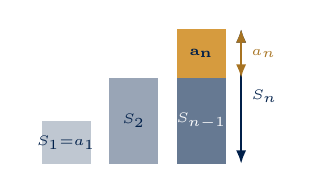
\begin{tikzpicture}[scale=0.78, line cap=round, line join=round]
  \fill[primary!25] (0.4,0) rectangle (1.2,0.7);
  \fill[primary!40] (1.5,0) rectangle (2.3,1.4);
  \fill[primary!60] (2.6,0) rectangle (3.4,2.2);
  \fill[gold!90] (2.6,1.4) rectangle (3.4,2.2);
  \node[font=\tiny\bfseries\color{primary}] at (0.8,0.35) {$S_1{=}a_1$};
  \node[font=\tiny\bfseries\color{primary}] at (1.9,0.7) {$S_2$};
  \node[font=\tiny\bfseries\color{white}] at (3.0,0.7) {$S_{n-1}$};
  \node[font=\tiny\bfseries\color{navy}] at (3.0,1.8) {$\mathbf{a_n}$};
  \draw[{Latex[scale=0.7]}-{Latex[scale=0.7]}, primary, line width=0.9pt] (3.65,0) -- (3.65,2.2) node[midway, right, font=\tiny\bfseries]{$S_n$};
  \draw[{Latex[scale=0.7]}-{Latex[scale=0.7]}, gold!80!black, line width=0.9pt] (3.65,1.4) -- (3.65,2.2) node[midway, right, font=\tiny\bfseries]{$a_n$};
\end{tikzpicture}
\end{minipage}\hfill
\begin{minipage}[c]{0.52\textwidth}
\begin{formulaBox}
  \textbf{The Bridge Formula:}
  $$\mathbf{a_n = S_n - S_{n-1} \quad (n \ge 2)}, \quad \mathbf{a_1 = S_1}$$
  \textbf{The Quadratic Signature of $S_n$:}
  $$S_n = \left(\frac{d}{2}\right)n^2 + \left(a - \frac{d}{2}\right)n = \mathbf{An^2 + Bn}$$
  \textbf{Speed Hacks for Board MCQs:}
  \begin{itemize}
    \item Common Difference: $\mathbf{d = 2A}$ (Twice coefficient of $n^2$)
    \item First Term: $\mathbf{a = A + B = S_1}$
    \item Constant Term: Must be \textbf{zero} for an AP from $n=1$.
  \end{itemize}
\end{formulaBox}
\end{minipage}

\vspace{0.8mm}
\subhead{6.2 Board Examination Protocol for $a_n = S_n - S_{n-1}$}

\begin{conceptBox}[title={Worked Archetype 6 $\vert$ Step-by-Step Derivation of $a_n$ from $S_n$},fonttitle=\bfseries\color{navy}]
  \textbf{Problem:} The sum of the first $n$ terms of an AP is $S_n = 3n^2 + 5n$. Find the $n$-th term and the $15$-th term.\\
  \textbf{Solution:}
  \begin{enumerate}
    \item \textbf{Express $S_{n-1}$:} Replace $n$ with $(n - 1)$:
      $$S_{n-1} = 3(n - 1)^2 + 5(n - 1) = 3(n^2 - 2n + 1) + 5n - 5 = 3n^2 - 6n + 3 + 5n - 5 = \mathbf{3n^2 - n - 2}$$
    \item \textbf{Apply Bridge Identity:}
      $$a_n = S_n - S_{n-1} = (3n^2 + 5n) - (3n^2 - n - 2) = 3n^2 + 5n - 3n^2 + n + 2 = \mathbf{6n + 2}$$
    \item \textbf{Boundary Check:} $a_1 = 6(1) + 2 = 8$. From formula, $S_1 = 3(1)^2 + 5(1) = 8$. Verified!
    \item \textbf{Find 15th Term:} $a_{15} = 6(15) + 2 = 90 + 2 = \mathbf{92}$.\\
      \textit{Verification Hack:} $S_n = 3n^2 + 5n \implies A=3, B=5 \implies d = 2(3) = 6, a = 3+5 = 8 \implies a_n = 6n + 2$.
  \end{enumerate}
\end{conceptBox}

\clearpage

% =============================================================================
% PAGE 8: MODULE 7 — THE DUAL ROOTS OF S_n = k: EXPLAINING DOUBLE ANSWERS
% =============================================================================
\thispagestyle{fancy}
\vspace*{0mm}

\chapterbanner{05}{ARITHMETIC PROGRESSIONS}{Module 7 $\vert$ The Dual Roots of $S_n = k$: Explaining Double Answers}{\CoreTag}

\subhead{7.1 The "Double Answer" Mechanism in Board Examinations}

When solving $S_n = k$, quadratic factorization frequently yields \textbf{two distinct natural numbers} $n = n_1$ and $n = n_2$ ($n_2 > n_1$).

\vspace{0.6mm}
\begin{minipage}[c]{0.45\textwidth}
\centering
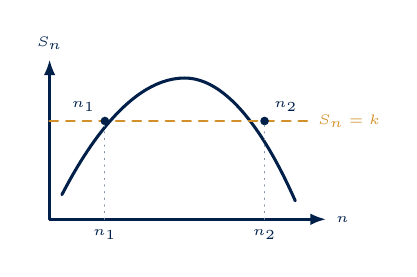
\begin{tikzpicture}[scale=0.78, line cap=round, line join=round]
  \draw[-{Latex[scale=0.8]}, primary, line width=0.9pt] (0,0) -- (4.5,0) node[right, font=\tiny\bfseries]{$n$};
  \draw[-{Latex[scale=0.8]}, primary, line width=0.9pt] (0,0) -- (0,2.6) node[above, font=\tiny\bfseries]{$S_n$};
  \draw[primary, line width=1.1pt] (0.2,0.4) parabola bend (2.2,2.3) (4.0,0.3);
  \draw[gold, line width=1pt, dashed] (0,1.6) -- (4.2,1.6) node[right, font=\tiny\bfseries\color{gold!90!black}]{$S_n = k$};
  \fill[reddeep] (0.9,1.6) circle (2pt) node[above left, font=\tiny\bfseries\color{reddeep}]{$n_1$};
  \fill[reddeep] (3.5,1.6) circle (2pt) node[above right, font=\tiny\bfseries\color{reddeep}]{$n_2$};
  \draw[dotted, primary!50] (0.9,0) -- (0.9,1.6);
  \draw[dotted, primary!50] (3.5,0) -- (3.5,1.6);
  \node[below, font=\tiny\bfseries\color{primary}] at (0.9,0) {$n_1$};
  \node[below, font=\tiny\bfseries\color{primary}] at (3.5,0) {$n_2$};
\end{tikzpicture}
\end{minipage}\hfill
\begin{minipage}[c]{0.52\textwidth}
\begin{formulaBox}
  \textbf{The Null-Sum Block Condition:}
  Two term counts $n_1$ and $n_2$ produce identical sums $S_{n_1} = S_{n_2} = k$ if and only if:
  $$\mathbf{\sum_{j = n_1 + 1}^{n_2} a_j = 0}$$
  \textbf{Mechanism:} Occurs when $a > 0$ and $d < 0$. The terms cross zero into negative values, and the negative terms cancel out the positive tail.
\end{formulaBox}
\end{minipage}

\vspace{0.8mm}
\subhead{7.2 Step-by-Step Classic Board Archetype}

\begin{conceptBox}[title={Worked Archetype 7 $\vert$ The Classic Double Root Board Model},fonttitle=\bfseries\color{navy}]
  \textbf{Problem:} How many terms of the AP: $24, 21, 18, \dots$ must be taken so that their sum is $78$? Explain the double answer.\\
  \textbf{Solution:}
  \begin{enumerate}
    \item Here, $a = 24$, $d = 21 - 24 = -3$, and $S_n = 78$.
    \item Sum equation:
      $$78 = \frac{n}{2}[2(24) + (n - 1)(-3)] \implies 156 = n[48 - 3n + 3] = n[51 - 3n] \implies 3n^2 - 51n + 156 = 0$$
    \item Dividing by $3$: $n^2 - 17n + 52 = 0 \implies (n - 4)(n - 13) = 0 \implies \mathbf{n = 4 \quad \text{or} \quad n = 13}$.
    \item \textbf{Board Explanation of Double Answer:}
      Both $n = 4$ and $n = 13$ are positive integers. The first $4$ terms sum to $24 + 21 + 18 + 15 = 78$.
      The remaining terms from $5$-th to $13$-th are:
      $$12 + 9 + 6 + 3 + 0 + (-3) + (-6) + (-9) + (-12) = \mathbf{0}$$
      Because this block sums to zero, adding them leaves the sum unchanged. Thus, \textbf{both answers are valid}.
  \end{enumerate}
\end{conceptBox}

\clearpage

% =============================================================================
% PAGE 9: MODULE 8 — PARAMETERIZED AP MODELS (p-th, q-th TERMS & VARIABLES)
% =============================================================================
\thispagestyle{fancy}
\vspace*{0mm}

\chapterbanner{05}{ARITHMETIC PROGRESSIONS}{Module 8 $\vert$ Parameterized AP Models: $p$-th, $q$-th Terms \& Unknown Constants}{\CoreTag}

\subhead{8.1 Universal Board Examination Identities}

\begin{tabularx}{\textwidth}{m{0.30\textwidth} | m{0.32\textwidth} | X}
\toprule
\rowcolor{bluepale}
\textbf{Given Hypothesis} & \textbf{Deduced Parameters ($a, d$)} & \textbf{Universal Board Result} \\
\midrule
$\mathbf{a_p = q}$ and $\mathbf{a_q = p}$ & $d = -1$, \quad $a = p + q - 1$ & $\mathbf{a_{p+q} = 0}$ \\
\midrule
$\mathbf{p \cdot a_p = q \cdot a_q} \quad (p \ne q)$ & $a + (p + q - 1)d = 0$ & $\mathbf{a_{p+q} = 0}$ \\
\midrule
$\mathbf{a_p = \frac{1}{q}}$ and $\mathbf{a_q = \frac{1}{p}}$ & $a = \frac{1}{pq}$, \quad $d = \frac{1}{pq}$ & $\mathbf{a_{pq} = 1}, \quad \mathbf{S_{pq} = \frac{1}{2}(pq + 1)}$ \\
\bottomrule
\end{tabularx}

\vspace{0.6mm}
\begin{minipage}[c]{0.45\textwidth}
\centering
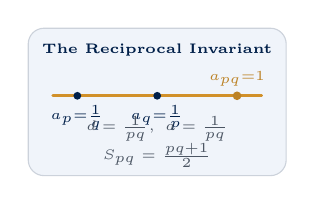
\begin{tikzpicture}[scale=0.78, line cap=round, line join=round]
  \draw[primary!20, fill=primarylight, rounded corners=2mm] (0,0) rectangle (4.2,2.4);
  \node[font=\tiny\bfseries\color{navy}] at (2.1,2.05) {The Reciprocal Invariant};
  \draw[line width=1pt, gold] (0.4,1.3) -- (3.8,1.3);
  \fill[primary] (0.8,1.3) circle (1.8pt) node[below, font=\tiny\bfseries]{$a_p{=}\frac{1}{q}$};
  \fill[primary] (2.1,1.3) circle (1.8pt) node[below, font=\tiny\bfseries]{$a_q{=}\frac{1}{p}$};
  \fill[gold!90!black] (3.4,1.3) circle (2pt) node[above, font=\tiny\bfseries\color{navy}]{$a_{pq}{=}1$};
  \node[font=\tiny\bfseries\color{secondary}, align=center] at (2.1,0.55) {$d = \frac{1}{pq}, \ a = \frac{1}{pq}$\\$S_{pq} = \frac{pq+1}{2}$};
\end{tikzpicture}
\end{minipage}\hfill
\begin{minipage}[c]{0.52\textwidth}
\begin{formulaBox}
  \textbf{Protocol for Unknown Variables:}
  If $f(x), g(x), h(x)$ are in AP:
  $$\mathbf{2 \cdot g(x) = f(x) + h(x)}$$
  $$\iff \mathbf{g(x) - f(x) = h(x) - g(x)}$$
  *Always equate consecutive differences directly!*
\end{formulaBox}
\end{minipage}

\vspace{0.8mm}
\subhead{8.2 Worked Algebraic Parameter Archetype}

\begin{conceptBox}[title={Worked Archetype 8 $\vert$ Unknown Parameter Determination},fonttitle=\bfseries\color{navy}]
  \textbf{Problem:} (i) If $a_p = \frac{1}{q}$ and $a_q = \frac{1}{p}$, prove $S_{pq} = \frac{1}{2}(pq + 1)$. (ii) Find $x$ such that $(x + 2), 2x, (2x + 3)$ are in AP.\\
  \textbf{Solution:}
  \begin{enumerate}
    \item State equations: $a + (p - 1)d = \frac{1}{q}$ and $a + (q - 1)d = \frac{1}{p}$. Subtracting:
      $$(p - q)d = \frac{1}{q} - \frac{1}{p} = \frac{p - q}{pq} \implies \mathbf{d = \frac{1}{pq}}, \quad \mathbf{a = \frac{1}{pq}}$$
      Now evaluate $S_{pq}$: $S_{pq} = \frac{pq}{2}\left[\frac{2}{pq} + (pq - 1)\frac{1}{pq}\right] = \frac{pq}{2}\left[\frac{pq + 1}{pq}\right] = \mathbf{\frac{pq + 1}{2}}$.
    \item For $(x + 2), 2x, (2x + 3)$ in AP: $2(2x) = (x + 2) + (2x + 3) \implies 4x = 3x + 5 \implies \mathbf{x = 5}$.
  \end{enumerate}
\end{conceptBox}

\clearpage

% =============================================================================
% PAGE 10: MODULE 9 — MASTER RATIO TRANSFORMATION & ADVANCED SUM RELATIONS
% =============================================================================
\thispagestyle{fancy}
\vspace*{0mm}

\chapterbanner{05}{ARITHMETIC PROGRESSIONS}{Module 9 $\vert$ The Master Ratio Transformation: Sum Ratios to Term Ratios}{\CoreTag}

\subhead{10.1 The Master Transformation Theorem}

Given the ratio of sums of two arithmetic progressions:
$$\mathbf{\frac{S_n}{S'_n} = \frac{f(n)}{g(n)}}$$
The ratio of their $\mathbf{m}$-th terms $\mathbf{\frac{a_m}{a'_m}}$ is obtained by replacing $\mathbf{n}$ with $\mathbf{(2m - 1)}$:
$$\mathbf{\frac{a_m}{a'_m} = \frac{f(2m - 1)}{g(2m - 1)}}$$

\vspace{0.6mm}
\begin{minipage}[c]{0.45\textwidth}
\centering
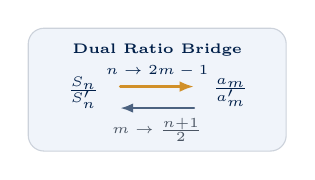
\begin{tikzpicture}[scale=0.78, line cap=round, line join=round]
  \draw[primary!20, fill=bluepale, rounded corners=2mm] (0,0) rectangle (4.2,2.0);
  \node[font=\tiny\bfseries\color{navy}] at (2.1,1.65) {Dual Ratio Bridge};
  \node[font=\tiny\bfseries\color{primary}] at (0.9,0.95) {$\frac{S_n}{S'_n}$};
  \node[font=\tiny\bfseries\color{reddeep}] at (3.3,0.95) {$\frac{a_m}{a'_m}$};
  \draw[{Latex[scale=0.7]}-, gold, line width=1pt] (2.7,1.05) -- (1.5,1.05);
  \node[font=\tiny\bfseries\color{navy}, above] at (2.1,1.05) {$n \to 2m-1$};
  \draw[-{Latex[scale=0.7]}, primary!70, line width=0.8pt] (2.7,0.7) -- (1.5,0.7);
  \node[font=\tiny\bfseries\color{secondary}, below] at (2.1,0.7) {$m \to \frac{n+1}{2}$};
\end{tikzpicture}
\end{minipage}\hfill
\begin{minipage}[c]{0.52\textwidth}
\begin{formulaBox}
  \textbf{Mathematical Proof of the $(2m - 1)$ Hack:}
  $$\frac{S_n}{S'_n} = \frac{\frac{n}{2}[2a_1 + (n - 1)d_1]}{\frac{n}{2}[2a_2 + (n - 1)d_2]} = \frac{a_1 + \left(\frac{n - 1}{2}\right)d_1}{a_2 + \left(\frac{n - 1}{2}\right)d_2}$$
  We require $\frac{a_1 + (m - 1)d_1}{a_2 + (m - 1)d_2}$. Equating coefficients:
  $$\frac{n - 1}{2} = m - 1 \implies \mathbf{n = 2m - 1}$$
\end{formulaBox}
\end{minipage}

\vspace{0.8mm}
\subhead{10.2 High-Scoring Board Archetype}

\begin{conceptBox}[title={Worked Archetype 9 $\vert$ Sum Ratio to Term Ratio Board Master},fonttitle=\bfseries\color{navy}]
  \textbf{Problem:} The ratio of the sums of $n$ terms of two arithmetic progressions is $(7n + 1) : (4n + 27)$. Find the ratio of their $11$-th terms.\\
  \textbf{Solution:}
  \begin{enumerate}
    \item State sum ratio: $\frac{S_n}{S'_n} = \frac{2a_1 + (n - 1)d_1}{2a_2 + (n - 1)d_2} = \frac{a_1 + \left(\frac{n - 1}{2}\right)d_1}{a_2 + \left(\frac{n - 1}{2}\right)d_2} = \frac{7n + 1}{4n + 27}$.
    \item We require the ratio of their $11$-th terms: $\frac{a_{11}}{a'_{11}} = \frac{a_1 + 10d_1}{a_2 + 10d_2}$.
    \item Set $\frac{n - 1}{2} = 10 \implies n - 1 = 20 \implies \mathbf{n = 21}$.
    \item Substitute $n = 21$ into the ratio:
      $$\frac{a_{11}}{a'_{11}} = \frac{7(21) + 1}{4(21) + 27} = \frac{147 + 1}{84 + 27} = \frac{148}{111} = \mathbf{\frac{4}{3}} \quad (\text{dividing by } 37)$$
      $\therefore$ The ratio of their $11$-th terms is \textbf{$4 : 3$}.
  \end{enumerate}
\end{conceptBox}

\clearpage

% =============================================================================
% PAGE 11: MODULE 10 — MASTER FORMULA MATRIX & DECISION ENGINE
% =============================================================================
\thispagestyle{fancy}
\vspace*{0mm}

\chapterbanner{05}{ARITHMETIC PROGRESSIONS}{Module 10 $\vert$ Master Formula Matrix \& Problem-Solving Decision Engine}{\ReferenceTag}

\subhead{11.1 Comprehensive Master Formula Matrix}

\begin{tabularx}{\textwidth}{m{0.22\textwidth} | m{0.34\textwidth} | X}
\toprule
\rowcolor{goldpale}
\textbf{Target Concept} & \textbf{Master Formula} & \textbf{Key Operational Conditions} \\
\midrule
\textbf{Common Difference} & $d = a_{k+1} - a_k$ & Constant for all $k \ge 1$; can be $>0, <0, =0$. \\
\midrule
\textbf{General Term ($n$-th)} & $a_n = a + (n - 1)d$ & $n \in \mathbb{N} = \{1, 2, 3, \dots\}$; linear polynomial $dn + (a-d)$. \\
\midrule
\textbf{$n$-th Term from End} & $a'_n = l - (n - 1)d$ & $l$ is last term; invariance: $a_n + a'_n = a + l$. \\
\midrule
\textbf{Middle Term(s)} & $k = \frac{m+1}{2}$ (odd $m$) & 1 term if $m$ is odd; 2 terms ($\frac{m}{2}, \frac{m}{2}+1$) if $m$ is even. \\
\midrule
\textbf{Arithmetic Mean} & $b = \frac{a+c}{2} \iff 2b = a+c$ & For 3 terms $a, b, c$ in AP. \\
\midrule
\textbf{Sum of $n$ Terms ($d$)} & $S_n = \frac{n}{2}[2a + (n - 1)d]$ & Quadratic in $n$ with zero constant: $An^2 + Bn$. \\
\midrule
\textbf{Sum of $n$ Terms ($l$)} & $S_n = \frac{n}{2}[a + l]$ & Deploy whenever last term $l = a_n$ is known. \\
\midrule
\textbf{Term from Sums} & $a_n = S_n - S_{n-1} \ (n \ge 2)$ & Always verify $a_1 = S_1$. Common difference $d = 2A$. \\
\bottomrule
\end{tabularx}

\vspace{0.8mm}
\subhead{11.2 Algorithmic Problem-Solving Decision Flowchart}

\centering
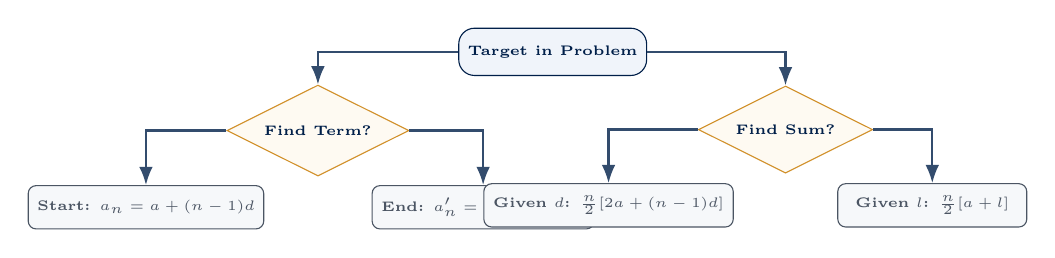
\begin{tikzpicture}[scale=0.82, auto, >=Latex,
    startstop/.style={rectangle, rounded corners=2mm, minimum width=2.0cm, minimum height=0.6cm, text centered, draw=primary, fill=primarylight, font=\tiny\bfseries\color{primary}},
    decision/.style={diamond, aspect=2, minimum width=2.0cm, minimum height=0.6cm, text centered, draw=gold, fill=goldpale, font=\tiny\bfseries\color{navy}},
    process/.style={rectangle, rounded corners=1mm, minimum width=2.4cm, minimum height=0.55cm, text centered, draw=secondary, fill=lightgray, font=\tiny\bfseries\color{secondary}},
    line/.style={draw=primary!80, line width=0.8pt, ->}]
    
  \node [startstop] (start) {Target in Problem};
  \node [decision, below left=0.4cm and 1.2cm of start] (t_term) {Find Term?};
  \node [decision, below right=0.4cm and 1.2cm of start] (t_sum) {Find Sum?};
  
  \node [process, below left=0.4cm and 0.1cm of t_term] (p_start) {Start: $a_n = a+(n-1)d$};
  \node [process, below right=0.4cm and 0.1cm of t_term] (p_end) {End: $a'_n = l-(n-1)d$};
  
  \node [process, below left=0.4cm and 0.1cm of t_sum] (p_sumd) {Given $d$: $\frac{n}{2}[2a+(n-1)d]$};
  \node [process, below right=0.4cm and 0.1cm of t_sum] (p_suml) {Given $l$: $\frac{n}{2}[a+l]$};
  
  \draw [line] (start) -| (t_term);
  \draw [line] (start) -| (t_sum);
  \draw [line] (t_term) -| (p_start);
  \draw [line] (t_term) -| (p_end);
  \draw [line] (t_sum) -| (p_sumd);
  \draw [line] (t_sum) -| (p_suml);
\end{tikzpicture}

\raggedright
\vspace{0.8mm}
\subhead{11.3 Standard Board Examination Presentation Protocol}

\begin{conceptBox}[title=Golden Rules for Securing 100\% Marks in Section C \& D,fonttitle=\bfseries\color{navy}]
  \begin{itemize}
    \item \textbf{Explicit Definitions:} Always state: \textit{"Let $a$ be the first term and $d$ be the common difference of the AP."}
    \item \textbf{Symbolic Formulas First:} Always write the general formula in standard algebraic symbols before plugging in numbers. CBSE marking schemes reserve $1/2$ mark specifically for the formula.
    \item \textbf{Integer Sanity Checks:} Whenever calculating $n$, explicitly state: \textit{"Since $n \in \mathbb{N}$, $n = \dots$ is accepted / rejected."}
  \end{itemize}
\end{conceptBox}

\clearpage

% =============================================================================
% PAGE 12: MODULE 11 — WORKED BOARD-EXAM MASTER ARCHETYPES
% =============================================================================
\thispagestyle{fancy}
\vspace*{0mm}

\chapterbanner{05}{ARITHMETIC PROGRESSIONS}{Module 11 $\vert$ Worked Board Exam Master Archetypes (Step-by-Step Rigor)}{\ExamTag}

\subhead{12.1 Archetype A: The First Negative Term Protocol (Inequality Method)}

\begin{conceptBox}[title={Board Model $\vert$ Finding the First Negative Term},fonttitle=\bfseries\color{navy}]
  \textbf{Problem:} Find the first negative term of the AP: $121, 117, 113, \dots$\\
  \textbf{Solution:}
  \begin{enumerate}
    \item Here, $a = 121$, $d = 117 - 121 = -4$. Set the strict inequality:
      $$a_n < 0 \implies 121 + (n - 1)(-4) < 0 \implies 121 - 4n + 4 < 0 \implies 125 < 4n \implies \mathbf{n > \frac{125}{4} = 31.25}$$
    \item Since $n$ must be the smallest natural number greater than $31.25$, we take $\mathbf{n = 32}$.
    \item \textbf{Value:} $a_{32} = 121 + 31(-4) = 121 - 124 = \mathbf{-3}$. The \textbf{$32$-nd term} is the first negative term.
  \end{enumerate}
\end{conceptBox}

\vspace{0.8mm}
\subhead{12.2 Archetype B: Multiples \& Divisibility in a Number Range}

\begin{conceptBox}[title={Board Model $\vert$ Sum of Divisible Numbers in a Given Interval},fonttitle=\bfseries\color{navy}]
  \textbf{Problem:} Find the sum of all natural numbers between $100$ and $500$ which are divisible by $7$.\\
  \textbf{Solution:}
  \begin{enumerate}
    \item Boundaries: Strictly $101 \le x \le 499$. First term $a = 105$, last term $l = 497$, difference $d = 7$.
    \item Number of terms: $497 = 105 + (n - 1)7 \implies 392 = 7(n - 1) \implies n - 1 = 56 \implies \mathbf{n = 57}$.
    \item Total sum: $S_{57} = \frac{57}{2}[a + l] = \frac{57}{2}[105 + 497] = \frac{57}{2}[602] = 57 \times 301 = \mathbf{17157}$.
  \end{enumerate}
\end{conceptBox}

\vspace{0.8mm}
\subhead{12.3 Archetype C: Symmetric 4-Term Ratio Model}

\begin{conceptBox}[title={Board Model $\vert$ 4 Terms with Ratio of Extremes to Means},fonttitle=\bfseries\color{navy}]
  \textbf{Problem:} Divide $32$ into four parts in AP such that the ratio of the product of extremes to the product of means is $7 : 15$.\\
  \textbf{Solution:}
  \begin{enumerate}
    \item Let the parts be $\mathbf{a - 3d, \ a - d, \ a + d, \ a + 3d}$ (Common difference $= 2d$).
    \item Sum: $(a - 3d) + (a - d) + (a + d) + (a + 3d) = 32 \implies 4a = 32 \implies \mathbf{a = 8}$.
    \item Ratio: $\frac{(8 - 3d)(8 + 3d)}{(8 - d)(8 + d)} = \frac{64 - 9d^2}{64 - d^2} = \frac{7}{15} \implies 15(64 - 9d^2) = 7(64 - d^2) \implies 960 - 135d^2 = 448 - 7d^2$.
    \item $512 = 128d^2 \implies d^2 = 4 \implies \mathbf{d = \pm 2}$. Taking $d = 2$, parts are: \textbf{$2, 6, 10, 14$}.
  \end{enumerate}
\end{conceptBox}

\clearpage

% =============================================================================
% PAGE 13: MODULE 12 — APPLIED CONTEXTUAL MODELING & CBSE CASE STUDIES
% =============================================================================
\thispagestyle{fancy}
\vspace*{0mm}

\chapterbanner{05}{ARITHMETIC PROGRESSIONS}{Module 12 $\vert$ Applied Contextual Modeling: Section E Case Studies}{\ExamTag}

\subhead{13.1 Case Study Archetype 1: The Semicircular Concentric Spiral}

A spiral is made up of successive semicircles with alternating centers at $A$ and $B$, of radii $r_1 = 0.5\text{ cm}, r_2 = 1.0\text{ cm}, r_3 = 1.5\text{ cm}, \dots$

\vspace{0.6mm}
\begin{minipage}[c]{0.52\textwidth}
\begin{conceptBox}[title=Mathematical Deconstruction,fonttitle=\bfseries\color{navy}]
  \begin{itemize}
    \item Semicircle length: $l_k = \pi r_k \implies l_1 = 0.5\pi, l_2 = 1.0\pi, \dots$
    \item Forms an AP with $a = 0.5\pi$ and $d = 0.5\pi$.
    \item \textbf{Total Length of 13 Semicircles ($n = 13$):}
      $$S_{13} = \frac{13}{2}[2(0.5\pi) + 12(0.5\pi)] = \frac{13}{2}[7\pi] = \frac{91}{2}\pi$$
      Using $\pi = \frac{22}{7}$: $S_{13} = \frac{91}{2} \times \frac{22}{7} = \mathbf{143\text{ cm}}$.
  \end{itemize}
\end{conceptBox}
\end{minipage}\hfill
\begin{minipage}[c]{0.45\textwidth}
\centering
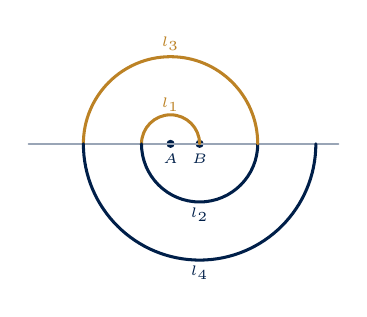
\begin{tikzpicture}[scale=0.82, line cap=round, line join=round]
  \coordinate (A) at (0,0);
  \coordinate (B) at (0.45,0);
  \fill[primary] (A) circle (1.8pt) node[below, font=\tiny\bfseries]{$A$};
  \fill[primary] (B) circle (1.8pt) node[below, font=\tiny\bfseries]{$B$};
  \draw[primary!40, line width=0.6pt] (-2.2,0) -- (2.6,0);

  \draw[gold!90!black, line width=1.1pt] (0.45,0) arc (0:180:0.45);
  \node[font=\tiny\bfseries\color{gold!90!black}] at (0,0.6) {$l_1$};

  \draw[primary, line width=1.1pt] (-0.45,0) arc (180:360:0.9);
  \node[font=\tiny\bfseries\color{primary}] at (0.45,-1.1) {$l_2$};

  \draw[gold!90!black, line width=1.1pt] (1.35,0) arc (0:180:1.35);
  \node[font=\tiny\bfseries\color{gold!90!black}] at (0,1.55) {$l_3$};

  \draw[primary, line width=1.1pt] (-1.35,0) arc (180:360:1.8);
  \node[font=\tiny\bfseries\color{primary}] at (0.45,-2.0) {$l_4$};
\end{tikzpicture}
\end{minipage}

\vspace{0.8mm}
\subhead{13.2 Case Study Archetype 2: The Potato Race / Retrieval Mechanics}

\begin{conceptBox}[title={Case Study Model $\vert$ The Potato Race Retrieval Mechanics},fonttitle=\bfseries\color{navy}]
  \textbf{Context:} A bucket is placed $5\text{ m}$ from the 1st potato. Other $9$ potatoes are spaced $3\text{ m}$ apart in a line ($10$ potatoes total). A competitor runs from the bucket, picks up each potato, and returns it to the bucket.\\
  \textbf{Step-by-Step Resolution:}
  \begin{enumerate}
    \item Distance for 1st potato $= 2 \times 5 = \mathbf{10\text{ m}}$. Distance for 2nd potato $= 2 \times (5 + 3) = \mathbf{16\text{ m}}$.
    \item Distances form an AP: $\mathbf{10, 16, 22, \dots}$ with $a = 10, d = 6$, and total terms $n = 10$.
    \item \textbf{Total Distance Run:} $S_{10} = \frac{10}{2}[2(10) + (10 - 1)6] = 5[20 + 54] = 5[74] = \mathbf{370\text{ meters}}$.
  \end{enumerate}
\end{conceptBox}

\vspace{0.8mm}
\subhead{13.3 Case Study Archetype 3: Production Scheduling \& Financial Installments}

A manufacturer produced $600$ cars in Year 3 and $700$ cars in Year 7 with uniform annual growth:
\begin{itemize}
  \item $a + 2d = 600$ and $a + 6d = 700 \implies 4d = 100 \implies \mathbf{d = 25\text{ cars/year}}$, First year: $a = \mathbf{550\text{ cars}}$.
  \item Production in Year 10: $a_{10} = a + 9d = 550 + 9(25) = \mathbf{775\text{ cars}}$.
  \item Total production in first 7 years: $S_7 = \frac{7}{2}[550 + 700] = 7 \times 625 = \mathbf{4375\text{ cars}}$.
\end{itemize}

\clearpage

% =============================================================================
% PAGE 14: MODULE 13 — BOARD EXAM TRAPS, HACKS & PRE-SUBMISSION AUDIT
% =============================================================================
\thispagestyle{fancy}
\vspace*{0mm}

\chapterbanner{05}{ARITHMETIC PROGRESSIONS}{Module 13 $\vert$ Board Traps, Verification Hacks \& 5-Point Audit}{\ExamTag}

\subhead{14.1 The Top 8 Arithmetic Progression Board Traps}

\begin{enumerate}[label=\textbf{Trap \arabic*:}, leftmargin=5mm, itemsep=0.8pt, topsep=0.6pt, parsep=0pt]
  \item \textbf{The Non-Integer Term Trap ($n \notin \mathbb{N}$):} Accepting fractional or negative values for $n$. Position index must strictly be a counting number: $\mathbf{n \in \{1, 2, 3, \dots\}}$. If $n = 23.4$, the term does NOT exist!
  \item \textbf{The "Between" vs "From" Interval Trap:} Numbers \textit{"between $100$ and $500$"} strictly \textbf{excludes} $100$ and $500$. Numbers \textit{"from $100$ to $500$"} \textbf{includes} $100$ and $500$ (if divisible).
  \item \textbf{The Common Difference Sign Reversal Trap:} In a decreasing AP ($20, 16, 12, \dots$), writing $d = 4$ instead of $\mathbf{d = -4}$. This completely reverses the signs of subsequent calculations!
  \item \textbf{The Symmetrical 4-Term Common Difference Error:} Selecting terms as $(a-3d, a-d, a+d, a+3d)$ and assuming the common difference is $d$. The actual common difference is $\mathbf{2d}$.
  \item \textbf{The Boundary Blindness Trap in $a_n = S_n - S_{n-1}$:} Attempting to calculate $a_1$ as $S_1 - S_0$. $S_0$ has no mathematical meaning in Class 10 AP. Always set $\mathbf{a_1 = S_1}$ directly!
  \item \textbf{The Distributive Factor Error in $S_n$:} Forgetting to distribute $\frac{n}{2}$ to both terms: writing $\frac{n}{2}[2a + (n-1)d]$ as $na + (n-1)d$. Always preserve the outer brackets!
  \item \textbf{The First Negative Term Inequality Sign Reversal:} In $-4n < -125$, forgetting to reverse the inequality sign when dividing by $-4$: writing $n < 31.25$ instead of $\mathbf{n > 31.25}$.
  \item \textbf{Confusing Position ($n$) with Value ($a_n$):} Mixing up the question \textit{"Which term is $78$?"} ($n = ?$) with \textit{"Find the $78$-th term"} ($a_{78} = ?$).
\end{enumerate}

\subhead{14.2 High-Speed Verification Hacks}

\begin{tabularx}{\textwidth}{X | X}
\toprule
\rowcolor{redpale}
\textbf{Traditional Slow Check (High Risk of Calculation Fatigue)} & \textbf{The Maths Manthan Instant Verification Hack} \\
\midrule
Verifying whether $S_n = 3n^2 + 5n$ yields an AP: & Look at the polynomial coefficients of $S_n = An^2 + Bn$: \\
Compute $S_1, S_2, S_3, S_4$. Find $a_1 = S_1, a_2 = S_2 - S_1, a_3 = S_3 - S_2$. Check if $a_3 - a_2 = a_2 - a_1$. & $\mathbf{d = 2A = 2(3) = 6}$ \\
Time taken: $\approx 3\text{ minutes}$. & $\mathbf{a = A + B = 3 + 5 = 8}$ \\
High risk of basic subtraction slip. & Instant check takes \textbf{3 seconds} with 100\% algebraic certainty! \\
\bottomrule
\end{tabularx}

\vspace{0.8mm}
\subhead{14.3 The 5-Point Board Examination Pre-Submission Checklist}

\begin{successBox}[top=1.2mm,bottom=1.2mm,before skip=1.2pt,after skip=1pt]
  \textbf{Final 60-Second Answer Sheet Verification Protocol:}
  \begin{itemize}[leftmargin=4mm,itemsep=0.8pt,topsep=0.8pt,parsep=0pt]
    \item[$\square$] \textbf{Domain Integrity Stated:} Did you verify that $n \in \mathbb{N}$ before accepting any value of $n$?
    \item[$\square$] \textbf{Symbolic Formula Declared:} Did you write $a_n = a + (n-1)d$ or $S_n = \frac{n}{2}[2a + (n-1)d]$ before substituting numeric values?
    \item[$\square$] \textbf{Sign of $d$ Verified:} If the series was decreasing, did you ensure $d$ was negative throughout?
    \item[$\square$] \textbf{Double Answer Justified:} For questions with two roots for $n$, did you explicitly explain that the intermediate terms sum to zero?
    \item[$\square$] \textbf{Physical Units Attached:} Are word problems and case studies concluded with correct physical units ($\text{meters}, \text{cars}, \text{cm}$)?
  \end{itemize}
\end{successBox}

\vfill
\begin{center}
  {\footnotesize\bfseries\color{primary}MATHS MANTHAN TUITION CLASSES \quad$\vert$\quad END OF CHAPTER 5 HANDBOOK}\\[1mm]
  {\scriptsize\color{secondary}Designed for Academic Excellence in CBSE Class 10 Board Examinations 2026--27.}
\end{center}

\end{document}
